% Created by tikzDevice version 0.10.1 on 2016-12-16 08:50:37
% !TEX encoding = UTF-8 Unicode
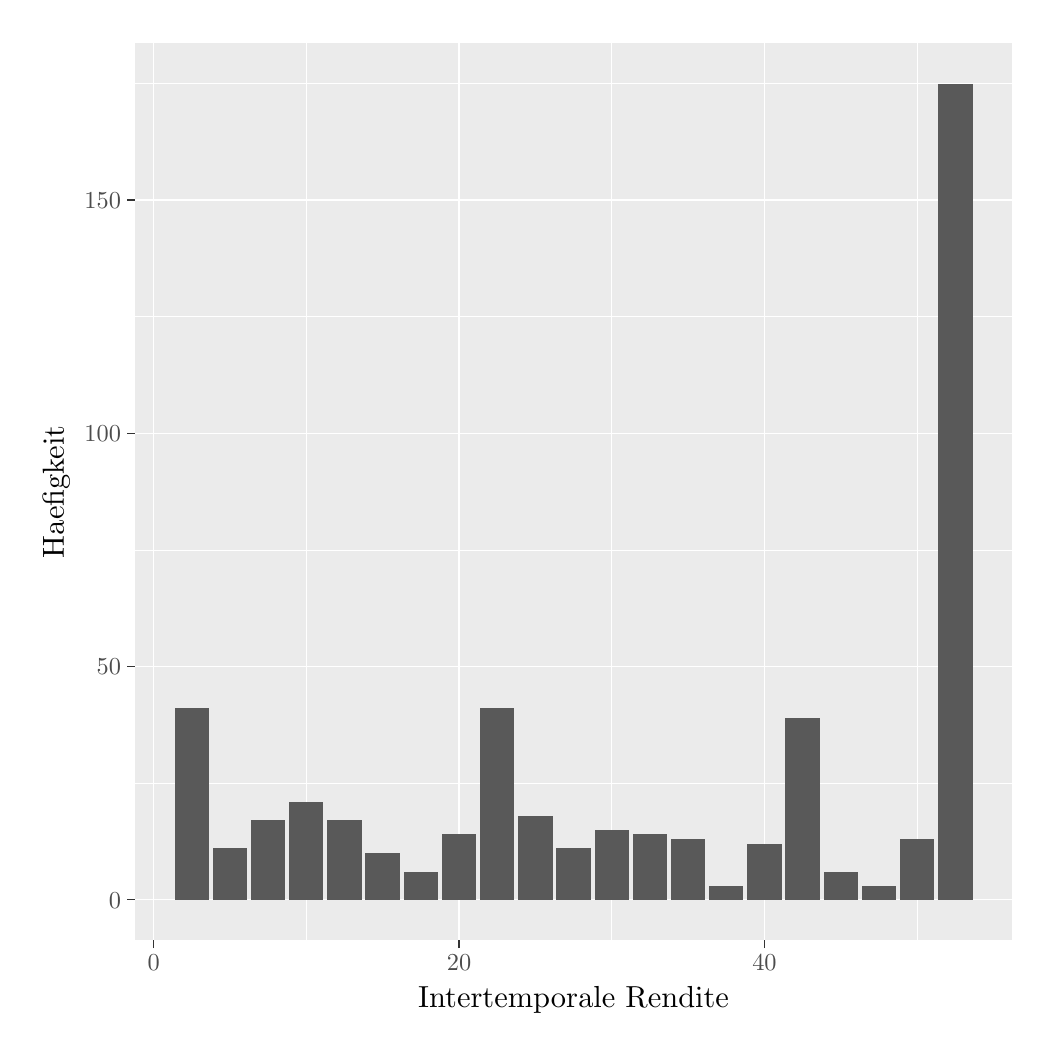
\begin{tikzpicture}[x=1pt,y=1pt]
\definecolor{fillColor}{RGB}{255,255,255}
\path[use as bounding box,fill=fillColor,fill opacity=0.00] (0,0) rectangle (361.35,361.35);
\begin{scope}
\path[clip] (  0.00,  0.00) rectangle (361.35,361.35);
\definecolor{drawColor}{RGB}{255,255,255}
\definecolor{fillColor}{RGB}{255,255,255}

\path[draw=drawColor,line width= 0.6pt,line join=round,line cap=round,fill=fillColor] (  0.00,  0.00) rectangle (361.35,361.35);
\end{scope}
\begin{scope}
\path[clip] ( 38.67, 31.53) rectangle (355.85,355.85);
\definecolor{fillColor}{gray}{0.92}

\path[fill=fillColor] ( 38.67, 31.53) rectangle (355.85,355.85);
\definecolor{drawColor}{RGB}{255,255,255}

\path[draw=drawColor,line width= 0.3pt,line join=round] ( 38.67, 88.39) --
	(355.85, 88.39);

\path[draw=drawColor,line width= 0.3pt,line join=round] ( 38.67,172.63) --
	(355.85,172.63);

\path[draw=drawColor,line width= 0.3pt,line join=round] ( 38.67,256.87) --
	(355.85,256.87);

\path[draw=drawColor,line width= 0.3pt,line join=round] ( 38.67,341.11) --
	(355.85,341.11);

\path[draw=drawColor,line width= 0.3pt,line join=round] (100.68, 31.53) --
	(100.68,355.85);

\path[draw=drawColor,line width= 0.3pt,line join=round] (211.05, 31.53) --
	(211.05,355.85);

\path[draw=drawColor,line width= 0.3pt,line join=round] (321.43, 31.53) --
	(321.43,355.85);

\path[draw=drawColor,line width= 0.6pt,line join=round] ( 38.67, 46.27) --
	(355.85, 46.27);

\path[draw=drawColor,line width= 0.6pt,line join=round] ( 38.67,130.51) --
	(355.85,130.51);

\path[draw=drawColor,line width= 0.6pt,line join=round] ( 38.67,214.75) --
	(355.85,214.75);

\path[draw=drawColor,line width= 0.6pt,line join=round] ( 38.67,298.99) --
	(355.85,298.99);

\path[draw=drawColor,line width= 0.6pt,line join=round] ( 45.50, 31.53) --
	( 45.50,355.85);

\path[draw=drawColor,line width= 0.6pt,line join=round] (155.87, 31.53) --
	(155.87,355.85);

\path[draw=drawColor,line width= 0.6pt,line join=round] (266.24, 31.53) --
	(266.24,355.85);
\definecolor{fillColor}{gray}{0.35}

\path[fill=fillColor] ( 53.08, 46.27) rectangle ( 65.50,115.35);

\path[fill=fillColor] ( 66.88, 46.27) rectangle ( 79.30, 64.81);

\path[fill=fillColor] ( 80.68, 46.27) rectangle ( 93.09, 74.91);

\path[fill=fillColor] ( 94.47, 46.27) rectangle (106.89, 81.65);

\path[fill=fillColor] (108.27, 46.27) rectangle (120.69, 74.91);

\path[fill=fillColor] (122.07, 46.27) rectangle (134.48, 63.12);

\path[fill=fillColor] (135.86, 46.27) rectangle (148.28, 56.38);

\path[fill=fillColor] (149.66, 46.27) rectangle (162.08, 69.86);

\path[fill=fillColor] (163.46, 46.27) rectangle (175.87,115.35);

\path[fill=fillColor] (177.25, 46.27) rectangle (189.67, 76.60);

\path[fill=fillColor] (191.05, 46.27) rectangle (203.47, 64.81);

\path[fill=fillColor] (204.85, 46.27) rectangle (217.26, 71.54);

\path[fill=fillColor] (218.64, 46.27) rectangle (231.06, 69.86);

\path[fill=fillColor] (232.44, 46.27) rectangle (244.86, 68.17);

\path[fill=fillColor] (246.24, 46.27) rectangle (258.65, 51.33);

\path[fill=fillColor] (260.03, 46.27) rectangle (272.45, 66.49);

\path[fill=fillColor] (273.83, 46.27) rectangle (286.25,111.98);

\path[fill=fillColor] (287.63, 46.27) rectangle (300.04, 56.38);

\path[fill=fillColor] (301.42, 46.27) rectangle (313.84, 51.33);

\path[fill=fillColor] (315.22, 46.27) rectangle (327.64, 68.17);

\path[fill=fillColor] (329.02, 46.27) rectangle (341.43,341.11);
\end{scope}
\begin{scope}
\path[clip] (  0.00,  0.00) rectangle (361.35,361.35);
\definecolor{drawColor}{gray}{0.30}

\node[text=drawColor,anchor=base east,inner sep=0pt, outer sep=0pt, scale=  0.88] at ( 33.72, 43.24) {0};

\node[text=drawColor,anchor=base east,inner sep=0pt, outer sep=0pt, scale=  0.88] at ( 33.72,127.48) {50};

\node[text=drawColor,anchor=base east,inner sep=0pt, outer sep=0pt, scale=  0.88] at ( 33.72,211.72) {100};

\node[text=drawColor,anchor=base east,inner sep=0pt, outer sep=0pt, scale=  0.88] at ( 33.72,295.96) {150};
\end{scope}
\begin{scope}
\path[clip] (  0.00,  0.00) rectangle (361.35,361.35);
\definecolor{drawColor}{gray}{0.20}

\path[draw=drawColor,line width= 0.6pt,line join=round] ( 35.92, 46.27) --
	( 38.67, 46.27);

\path[draw=drawColor,line width= 0.6pt,line join=round] ( 35.92,130.51) --
	( 38.67,130.51);

\path[draw=drawColor,line width= 0.6pt,line join=round] ( 35.92,214.75) --
	( 38.67,214.75);

\path[draw=drawColor,line width= 0.6pt,line join=round] ( 35.92,298.99) --
	( 38.67,298.99);
\end{scope}
\begin{scope}
\path[clip] (  0.00,  0.00) rectangle (361.35,361.35);
\definecolor{drawColor}{gray}{0.20}

\path[draw=drawColor,line width= 0.6pt,line join=round] ( 45.50, 28.78) --
	( 45.50, 31.53);

\path[draw=drawColor,line width= 0.6pt,line join=round] (155.87, 28.78) --
	(155.87, 31.53);

\path[draw=drawColor,line width= 0.6pt,line join=round] (266.24, 28.78) --
	(266.24, 31.53);
\end{scope}
\begin{scope}
\path[clip] (  0.00,  0.00) rectangle (361.35,361.35);
\definecolor{drawColor}{gray}{0.30}

\node[text=drawColor,anchor=base,inner sep=0pt, outer sep=0pt, scale=  0.88] at ( 45.50, 20.52) {0};

\node[text=drawColor,anchor=base,inner sep=0pt, outer sep=0pt, scale=  0.88] at (155.87, 20.52) {20};

\node[text=drawColor,anchor=base,inner sep=0pt, outer sep=0pt, scale=  0.88] at (266.24, 20.52) {40};
\end{scope}
\begin{scope}
\path[clip] (  0.00,  0.00) rectangle (361.35,361.35);
\definecolor{drawColor}{RGB}{0,0,0}

\node[text=drawColor,anchor=base,inner sep=0pt, outer sep=0pt, scale=  1.10] at (197.26,  7.44) {Intertemporale Rendite};
\end{scope}
\begin{scope}
\path[clip] (  0.00,  0.00) rectangle (361.35,361.35);
\definecolor{drawColor}{RGB}{0,0,0}

\node[text=drawColor,rotate= 90.00,anchor=base,inner sep=0pt, outer sep=0pt, scale=  1.10] at ( 13.08,193.69) {Haefigkeit};
\end{scope}
\end{tikzpicture}
